% Created 2020-07-16 jue 13:26
% Intended LaTeX compiler: pdflatex
\documentclass[presentation,aspectratio=169]{beamer}
\usepackage[utf8]{inputenc}
\usepackage[T1]{fontenc}
\usepackage{graphicx}
\usepackage{grffile}
\usepackage{longtable}
\usepackage{wrapfig}
\usepackage{rotating}
\usepackage[normalem]{ulem}
\usepackage{amsmath}
\usepackage{textcomp}
\usepackage{amssymb}
\usepackage{capt-of}
\usepackage{hyperref}
\usepackage{khpreamble}
\usepackage{amssymb}
\DeclareMathOperator{\shift}{q}
\DeclareMathOperator{\diff}{p}
\usetheme{default}
\author{Kjartan Halvorsen}
\date{\today}
\title{Control computarizado - Asignación de polos, controlador incremental}
\hypersetup{
 pdfauthor={Kjartan Halvorsen},
 pdftitle={Control computarizado - Asignación de polos, controlador incremental},
 pdfkeywords={},
 pdfsubject={},
 pdfcreator={Emacs 26.3 (Org mode 9.3.6)}, 
 pdflang={English}}
\begin{document}

\maketitle

\section{Intro}
\label{sec:orgb4a86e5}
\section{2-dof controller}
\label{sec:org21976d4}
\begin{frame}[label={sec:org4290b8b}]{Controlador de dos grados de libertad}
\begin{center}
\includegraphics[width=0.7\linewidth]{../../figures/2dof-block-explicit}
\end{center}
\end{frame}
\section{Problem 5.3}
\label{sec:org572b93a}
\begin{frame}[label={sec:org7fb08d9}]{Åström \& Wittenmark problema 5.3}
Dado sistema
\[ H(z) = \frac{z+0.7}{z^2 -1.8z + 0.81} \]
Determina controlador de dos grados de libertad, dónde el polinomio caracteristica del sistema en lazo cerrado, desde la señal de referencia a la salida sea
\[ A_c(z) = z^2 - 1.5z + 0.7. \]
Pon los polos del observador en el origen (deadbeat observer). Considera tres casos
\begin{description}
\item[{(a)}] Control posicional \alert{con} cancelación del cero del proceso
\item[{(b)}] Control posicional \alert{sin} cancelación del cero del proceso
\item[{(c)}] Control \alert{incremental} sin cancelación del cero del proceso
\end{description}
\end{frame}

\begin{frame}[label={sec:org6c9fe00}]{¿Por qué cancelar el cero?}
Diagramas de Bode para los sistemas en lazo cerrado (seguimiento de referencia) con y sin cancelación del cero

\begin{center}
\includegraphics[width=0.6\linewidth]{../../figures/aw5_3_bode}
\end{center}
\end{frame}

\begin{frame}[label={sec:orge808125}]{Ejercicio preliminario 1}
Dado sistema \(H(z) = \frac{z+0.7}{z^2 -1.8z + 0.81}\) y polinomio caracteristico deseado \(A_c(z) = z^2 - 1.5z + 0.7\)

\alert{Actividad} Marca los polos del proceso \(H(z)\), y los polos deseados del sistema en lazo cerrado, asumiendo \(h=0.1\).

\begin{center}
\alert{plano s} \hspace*{0.4\linewidth} \alert{plano z}\\
\includegraphics[height=0.56\textheight]{../../figures/sgrid-crop} \hspace*{3mm}
\includegraphics[height=0.55\textheight]{../../figures/zgrid-crop}\\
\end{center}
\end{frame}

\begin{frame}[label={sec:org7ef679f}]{Ejercicio preliminario 1 - Solución}
Dado sistema \(H(z) = \frac{z+0.7}{z^2 -1.8z + 0.81} = \frac{z+0.7}{(z-0.9)^2}\) y polinomio caracteristico deseado \(A_c(z) = z^2 - 1.5z + 0.7 = (z - 0.75 + i0.37)(z-0.75 - i 0.37)\).
\begin{center}
  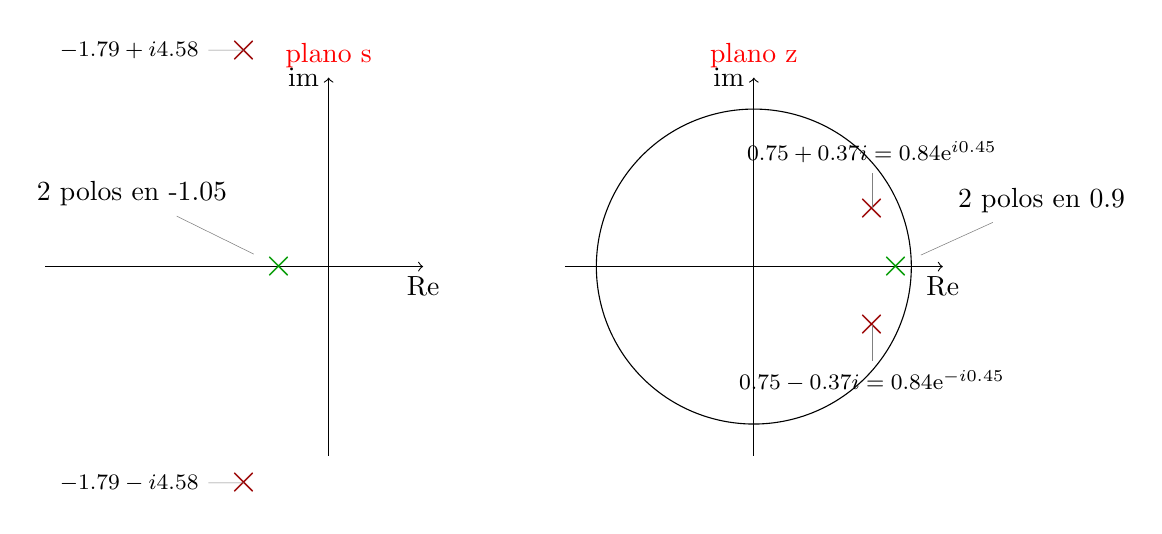
\begin{tikzpicture}
    \begin{scope}[scale=2]
      \draw[->] (-1.2, 0) to (1.2, 0) node[below] {Re};
      \draw[->] (0,-1.2) to (0,1.20) node[left] {im} node[above, red] {plano z};
      \draw[domain=0:360, samples=361] plot ({cos(\x)}, {sin(\x)});
      \node[green!60!black, pin=40:{2 polos en 0.9}] at (0.9, 0) {\Large $\times$};
      \node[red!60!black] at (0.75, 0.37) {\Large $\times$};
      \node[coordinate, pin=90:{\footnotesize $0.75+0.37i = 0.84\mathrm{e}^{i0.45}$}] at (0.75, 0.37) {};

      \node[red!60!black] at (0.75, -0.37) {\Large $\times$};
      \node[coordinate, pin=-90:{\footnotesize $0.75-0.37i = 0.84\mathrm{e}^{-i0.45}$}] at (0.75, -0.37) {};
    \end{scope}

    \begin{scope}[scale=0.6, xshift=-9cm]
      \draw[->] (-6, 0) to (2, 0) node[below] {Re};
      \draw[->] (0,-4) to (0,4) node[left] {im} node[above, red] {plano s};
      \node[green!60!black, pin=130:{2 polos en -1.05}] at (-1.05, 0) {\Large $\times$};
      \node[red!60!black] at (-1.79, 4.58) {\Large $\times$};
      \node[coordinate, pin=180:{\footnotesize $-1.79 + i4.58$}] at (-1.79, 4.58) {};
      \node[red!60!black] at (-1.79, -4.58) {\Large $\times$};
      \node[coordinate, pin=180:{\footnotesize $-1.79 - i4.58$}] at (-1.79, -4.58) {};
    \end{scope}

  \end{tikzpicture}
\end{center}
\end{frame}

\begin{frame}[label={sec:org6ae4e2c}]{Ejercicio preliminario 2}
Cuál de las respuestas de sistema en lazo cerrado corresponde a (I) Control posicional \alert{con} cancelación del cero del proceso,  (II) Control posicional \alert{sin} cancelación del cero del, (III) Control \alert{incremental} sin cancelación del cero del proceso
\begin{center}
\includegraphics[width=0.45\linewidth]{../../figures/aw5_3_refstep}
\includegraphics[width=0.45\linewidth]{../../figures/aw5_3_diststep}
\end{center}
\end{frame}

\begin{frame}[label={sec:org1bc8b80}]{Asignación de los polos}
\end{frame}

\section{Caso (a)}
\label{sec:orgc706865}
\begin{frame}[label={sec:org3b73bab}]{Caso (a) Controlador posicional con cancelación del cero}
Dado sistema \(H(z) = \frac{z+0.7}{z^2 -1.8z + 0.81}\) y polinomio caracteristico deseado
\(A_c(z) = z^2 - 1.5z + 0.7.\)

\begin{enumerate}
\item \alert{Orden del controlador} Eligimos el controlador \[F_b(z) = \frac{S(z)}{R(z)} = \frac{S(z)}{(z+1)\bar{R}(z)}\]
 para que haya cancelación del cero. Ecuación diofantina
\[A(z)(z+0.7)\bar{R}(z) + (z+0.7)S(z) = (z+0.7)A_c(z)A_o(z)\]
\[A(z)\bar{R}(z) + S(z) = A_c(z)A_o(z) \qquad (*)\]
Número de coeficientes desconocidos del controlador: \(n_{\bar{R}} + n_{\bar{R}} +  2\).
Número de ecuaciones de la ecuación diofantina: \(n_A + n_{\bar{R}}\).
\alert{\(\Rightarrow\qquad \(n_{\bar{R}} = n_{A} - 2 = 2-2 = 0\)}
\[ F_{b}(z) = \frac{s_0z + s_1}{z+0.7}\]
\end{enumerate}
\end{frame}
\begin{frame}[label={sec:org4bbb021}]{Caso (a) Controlador posicional con cancelación del cero}
\begin{enumerate}
\setcounter{enumi}{1}
\item \alert{Polinomio del obervador} Factorización de \(A_{cl}(z) = A_c(z)A_o(z)\). Ecuación \((*)\) es de orden 2, igual  que \(A_c(z)\), entonces \alert{\[A_o(z) = 1\]}.
\end{enumerate}
\end{frame}

\begin{frame}[label={sec:org2f5ddde}]{Caso (a) Controlador posicional con cancelación del cero}
\begin{enumerate}
\setcounter{enumi}{2}
\item \alert{Solución de la ecuación diofantina} Determina los polinomios \(R(z)\) y \(S(z)\). La ecuación diofantina
\[ (z^2 - 1.8z + 0.81) + s_0z + s_1 = z^2 - 1.5z + 0.7 \]
nos da el sistema de ecuaciones
\[ \begin{cases} z^1 :&  s_0 = -1.5+1.8= 0.3\\ z^0:& s_1 = 0.7-0.81=-0.11 \end{cases}\]
\alert{\[F_b(z) = \frac{0.3z - 0.11}{z + 0.7}\]}
\end{enumerate}
\end{frame}
\begin{frame}[label={sec:org7ab64d0}]{Caso (a) Controlador posicional con cancelación del cero}
\begin{enumerate}
\setcounter{enumi}{3}
\item \alert{El polinomio \(T(z)\)}  \[F_f(z) = \frac{T(z)}{R(z)} = \frac{t_0 A_o(z)}{B(z)}\]
Función de transferencia del seguimiento a la referencia:
\[ G_c(z) = \frac{ \frac{T}{R}\frac{B}{A}}{1 + \frac{B}{A} \frac{S}{R}} = 
                  = \frac{TB}{AR+BS} = \frac{t_0B}{BA_c} = \frac{t_0}{A_c(z)}\]
Para obtener ganancia stática unitaria:
  \alert{\[ t_0 = A_c(1) = 0.2 \]}
\end{enumerate}

Controlador completo

\begin{align*}
U(z) &= \frac{T(z)}{R(z}U_c(z) - \frac{S(z)}{R(z)}Y(z) = \frac{0.2}{z+0.7}U_c(z) - \frac{0.3z - 0.11}{z+0.7} Y(z)
     \end{align*}
\end{frame}

\section{Caso (c)}
\label{sec:org67f5d4d}
\begin{frame}[label={sec:org8fd4c31}]{Caso (c) Controlador incremental sin cancelación del cero}
Dado sistema
\[ H(z) = \frac{z+0.7}{z^2 -1.8z + 0.81} \]
y polinomio caracteristico deseado
\[ A_c(z) = z^2 - 1.5z + 0.7. \]

\begin{enumerate}
\item \alert{Orden del controlador}  \(F_b(z) = \frac{S(z)}{(z-1)\bar{R}(z)}\), con \(n_S = n_{\bar{R}} + 1\) nos da la ecuación diofantina
\[ A(z)(z-1)\bar{R}(z) + B(z)S(z) = A_c(z)A_o(z)\]
Número de coeficientes desconocidos del controlador: \(n_{\bar{R}} + \n_{\bar{R}} + 2\).
Número de ecuaciones de la ecuación diofantina: \(n_A + n_\bar{R} + 1\).
\alert{\(\Rightarrow\qquad \(n_{\bar{R}} = n_{A} + 1- 2 = 1\)}
\[ F_{b}(z) = \frac{s_0z^2 + s_1z + s_2 }{(z-1)(z+r_1)}\]
\end{enumerate}
\end{frame}


\begin{frame}[label={sec:orga8f2838}]{Caso (c) Controlador incremental sin cancelación del cero}
\begin{enumerate}
\setcounter{enumi}{1}
\item \alert{Polinomio del obervador} Factorización de \(A_{cl}(z) = A_c(z)A_o(z)\). La ecuación diofantina es de orden 4, y tenemos el polinomio caracteristico deseado \(A_c(z) = z^2 -1.5z + 0.7\). Entonces \alert{\[A_o(z) = z^2\]}
\end{enumerate}
\end{frame}

\begin{frame}[label={sec:org031f03b}]{Caso (c) Controlador incremental sin cancelación del cero}
\begin{enumerate}
\setcounter{enumi}{2}
\item \alert{Solución de la ecuación diofantina} 
\[(z^2 - 1.8z + 0.81)(z-1)(z+r_1) + (z+0.7)(s_0z^2 + s_1z + s_2) = z^2(z^2-1.5z+0.7) \]
\begin{itemize}
\item El lado izqierdo
\[(z^2 - 1.8z + 0.81)(z^2 +(r_1-1)z - r_1) + s_0z^3 + s_1z^2 + s_2z + 0.7s_0z^2 + 0.7s_1z + 0.7s_2\] 
\[z^4 - 1.8z^3 + 0.81z^2 + (r_1-1)z^3 - 1.8(r_1-1)z^2 + 0.81(r_1-1)z - r_1z^2 + 1.8r_1z - 0.81r_1 \]
\begin{multline*}
z^4 + (r_1 + s_0 -2.8)z^3 + (-2.8r_1 + 0.7s_0 + s_1 +2.61)z^2 + (2.61 r_1 + 0.7s_1 + s_2 -0.81)z\\   + (-0.81r_1 + 0.7s_2)\end{multline*}
\end{itemize}
\end{enumerate}
\end{frame}

\begin{frame}[label={sec:org3a84065}]{Caso (c) Controlador incremental sin cancelación del cero}
\begin{enumerate}
\setcounter{enumi}{2}
\item \alert{Solución de la ecuación diofantina} 
\begin{multline*}
  z^4 + (r_1 + s_0 -2.8)z^3 + (-2.8r_1 + 0.7s_0 + s_1 +2.61)z^2 + (2.61 r_1 + 0.7s_1 + s_2 -0.81)z\\   + (-0.81r_1 + 0.7s_2) = z^4 -1.5z^3 + 0.7z^2\end{multline*} 
Coeficientes iguales da las ecuaciones
\[ \begin{cases} z^3: & r_1 + s_0 = 2.8 -1.5\\
              z^2: & -2.8 r_1 + 0.7s_0 + s_1 = -2.61 +0.7\\
              z^1: &  2.61r_1 + 0.7s_1 + s_2 = 0.81\\
              z^0: & -0.81r_1 + 0.7s_2 = 0  \end{cases} \]

\alert{\[ R(z) = (z-1)(z + 0.45), \qquad S(z) = 0.85z^2 - 1.25z + 0.52\]}
\end{enumerate}
\end{frame}

\begin{frame}[label={sec:org332aab3}]{Caso (c) Controlador incremental sin cancelación del cero}
\begin{enumerate}
\setcounter{enumi}{3}
\item \alert{El polinomio \(T(z)\)}  \[F_f(z) = \frac{T(z)}{R(z)} = \frac{t_0 A_o(z)}{B(z)}, \qquad G_c(z) = \frac{t_0 B(z)}{A_c(z)}, \qquad G_(1) = 1 \quad\Rightarrow \]
\alert{\[ t_0 = \frac{A_c(1)}{B(1)} = \frac{1 - 1.5 + 0.7}{1+0.7} = \frac{2}{17}\]}
\end{enumerate}

Controlador completo

\begin{align*}
U(z) &= \frac{T(z)}{R(z}U_c(z) - \frac{S(z)}{R(z)}Y(z) \\
     &= \frac{\frac{2}{17}z^2}{(z-1)(z+0.45)}U_c(z) - \frac{0.85z^2 - 1.25z + 0.52}{(z-1)(z+0.45)} Y(z)
     \end{align*}
\end{frame}

\begin{frame}[label={sec:orgda48ef9}]{La importancia de los polos del observador}
\href{https://mybinder.org/v2/gh/kjartan-at-tec/mr2007-computerized-control/master?filepath=.\%2Fpolynomal-design/notebooks/A-and-W-5.3.ipynb}{Mybinder}
\end{frame}
\end{document}